% 第 8 题点列图：按固定源 PDF 矢量路径换算（1 pt → 0.03515 cm）。
% 原点取下边水平线的左端（源页 (533.34, 203.23) pt），y 向上。
% 两条边（角的两边）：水平线 y=0 与斜线（自 (0.37,20.99) 至 (103.90,78.47)）；
% 角的顶点在图外有意未绘出（两线左端被同一竖直截断线切齐，端头纵向相距 20.99 pt）。
% 三个 10% 灰填充三角形 S1/S2/Sn（顶点按源路径逐点换算）；
% 点列 A1..A(n+1) 在斜线上、B1..B(n+1) 在水平线上；4 组省略号（A 线 1、S 行 2、B 行 1）。
% 全部标签按源字形框中心显式坐标定位。
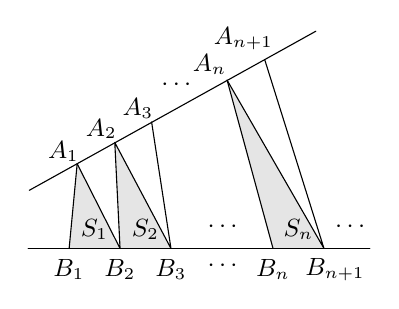
\begin{tikzpicture}[line cap=round,line join=round,font=\small,x=0.03515cm,y=0.03515cm]
% ===== 两条边 =====
\draw (0,0)--(123.43,0);               % 水平线（下边，B 点列所在）
\draw (0.37,20.99)--(103.90,78.47);    % 斜线（上边，A 点列所在）
% ===== 填充三角形（fill-opacity 0.1）=====
\fill[black,fill opacity=0.1] (17.68,30.58)--(14.78,-0.01)--(33.17,-0.01)--cycle;
\fill[black,fill opacity=0.1] (31.27,38.28)--(33.17,-0.01)--(51.56,-0.01)--cycle;
\fill[black,fill opacity=0.1] (71.84,60.79)--(88.43,0.01)--(106.83,0.01)--cycle;
% ===== 线段 =====
\draw (17.68,30.58)--(14.78,-0.01);                       % A1B1
\draw (17.68,30.58)--(33.17,-0.01)--(31.27,38.28)--(51.56,-0.01)--(44.57,45.68);  % A1→B2→A2→B3→A3
\draw (71.84,60.79)--(88.43,0.01);                        % AnBn
\draw (71.84,60.79)--(106.83,0.01)--(85.43,68.19);        % An→Bn+1→An+1
% ===== 标签（照源字形框中心，显式坐标）=====
\node[anchor=center,inner sep=0] at (12.71,34.93) {\(A_{1}\)};
\node[anchor=center,inner sep=0] at (26.35,43.11) {\(A_{2}\)};
\node[anchor=center,inner sep=0] at (39.62,50.48) {\(A_{3}\)};
\node[anchor=center,inner sep=0] at (53.51,59.21) {\(\cdots\)};
\node[anchor=center,inner sep=0] at (65.48,66.56) {\(A_{n}\)};
\node[anchor=center,inner sep=0] at (77.72,75.76) {\(A_{n+1}\)};
\node[anchor=center,inner sep=0] at (14.70,-7.57) {\(B_{1}\)};
\node[anchor=center,inner sep=0] at (33.12,-7.57) {\(B_{2}\)};
\node[anchor=center,inner sep=0] at (51.55,-7.57) {\(B_{3}\)};
\node[anchor=center,inner sep=0] at (70.23,-6.14) {\(\cdots\)};
\node[anchor=center,inner sep=0] at (88.41,-7.57) {\(B_{n}\)};
\node[anchor=center,inner sep=0] at (110.82,-7.57) {\(B_{n+1}\)};
\node[anchor=center,inner sep=0] at (23.91,6.82) {\(S_{1}\)};
\node[anchor=center,inner sep=0] at (42.34,6.82) {\(S_{2}\)};
\node[anchor=center,inner sep=0] at (70.23,7.81) {\(\cdots\)};
\node[anchor=center,inner sep=0] at (97.63,6.82) {\(S_{n}\)};
\node[anchor=center,inner sep=0] at (116.30,7.81) {\(\cdots\)};
\end{tikzpicture}
